\chapter{Methodology}
\label{chapter:methodology}

This section describes, in detail, the methodology behind this dissertation's research objectives, namely:

\begin{itemize}
    \item Dataset description, preprocessing steps, and augmentation techniques;
    \item Software stack used to describe said experiments in code;
    \item Computational resources used to execute the experiments.
\end{itemize}

\section{Data}

The \ac{ISIC} 2017: Skin Lesion Analysis Towards Melanoma Detection grand challenge datasets \cite{isic2017} provides a training set with 2000 samples (divided into three classes: 374 melanoma, 254 seborrheic keratosis, and 1372 nevus), a validation set with 150 samples, and a test set with 600 samples. However training deep neural networks for skin lesion classification requires vast amounts of high quality, reliably labeled and verified data - a set of requirements which this dataset did not meet with confidence.

The \ac{HAM10000} \cite{ham10000} dataset is an effort to boost research on automated diagnosis of dermatoscopic images that focuses on the quality and reliability of the large volume of data that is so important for successful deep learning. The extracted images (where the lesion is centered if necessary) go through an extensive semi-automatic process that filters out non-dermoscopic imaging and unreliable diagnoses, after which they are submitted to a manual review to further confirm its quality.

The datasets from the \ac{ISIC} 2018 grand challenge \cite{isic2018} were largely based on \ac{HAM10000} that was already very high quality, which meant the data preprocessing needs would be much lower compared to the previous years' editions where all these quality guarantees had to be independently ensured by the competitors. The \ac{ISIC} 2018 datasets are therefore adequate for running these experiments.

\subsection{Preprocessing}
\label{subsection:preprocessing}

The images in the dataset undergo a number of preprocessing steps:

\begin{enumerate}
    \item Most readily available pretrained models are of network architectures whose input tensor is of square dimensions (e.g. $224 \times 224 \times 3$). Since our dataset's images are of distinct non-square dimensions, it is necessary to resize them to a square. However, resizing them all naively to the network's input tensor dimensions without regards to the image's aspect ratio means that the input fed to the network is of varying distinct aspect ratios which does not constitute a good start. Therefore, the first step is to crop an arbitrarily-sized square of the center of the image which will likely (and, in fact, does) capture the skin lesion.

    \begin{listing}[ht]
    \begin{minted}{python}
    def _crop(img):
        width, height = img.size
        if width == height:
            return img

        length = min(width, height)

        left = (width - length) // 2
        upper = (height - length) // 2
        right = left + length
        lower = upper + length

        box = (left, upper, right, lower)
        return img.crop(box)
    \end{minted}
    \caption{Function that crops a given image to a square crop of the center of the original image.}
    \label{code:crop}
    \end{listing}

\item Resize the images to the target networks' input dimensions $224 \times 224 \times 3$ and $299 \times 299 \times 3$. We resize them as soon as possible in the data pipeline in order to reduce the computational costs of any subsequent operations on the images.

    \begin{listing}[ht]
    \begin{minted}{python}
    def _resize(img, target_size):
        return img.resize(target_size, PIL.Image.NEAREST)
    \end{minted}
    \caption{Function that resizes a given image to the target dimensions.}
    \label{code:resize}
    \end{listing}

    \item Normalize the luminance and apply a 99\% contrast stretch to reduce the negative effect of changes in illumination and acquisition devices that alter the color of images \cite{colorconstancy}.

    \begin{listing}[ht]
    \begin{minted}{python}
    def _correct(img):
        img_y, img_b, img_r = img.convert('YCbCr').split()

        img_y_np = np.asarray(img_y).astype(float)

        img_y_np /= 255
        img_y_np -= img_y_np.mean()
        img_y_np /= img_y_np.std()
        scale = np.max([np.abs(np.percentile(img_y_np, 1.0)),
                        np.abs(np.percentile(img_y_np, 99.0))])
        img_y_np = img_y_np / scale
        img_y_np = np.clip(img_y_np, -1.0, 1.0)
        img_y_np = (img_y_np + 1.0) / 2.0

        img_y_np = (img_y_np * 255 + 0.5).astype(np.uint8)

        img_y = PIL.Image.fromarray(img_y_np)

        img_ybr = PIL.Image.merge('YCbCr', (img_y, img_b, img_r))
        return img_ybr.convert('RGB')
    \end{minted}
    \caption{Function that normalizes the luminance of an image and applies a 99\% contrast stretch.}
    \label{code:correct}
    \end{listing}
\end{enumerate}

\subsection{Augmentation}
\label{subsection:augmentation}

In our binary classification task (melanoma vs non-melanoma) the $m = 10015$ samples in the training set are highly imbalanced (illustrated in figure \ref{fig:classimbalance}):

\begin{itemize}
    \item the majority class has $|S_{maj}| = 8902$ samples, constituting $\frac{8902}{10015} \times 100 = 88.9\%$ of the samples;
    \item the minority class has $|S_{min}| = 1113$ samples, constituting $\frac{1113}{10015} \times 100 = 11.1\%$ of the samples.
\end{itemize}

\begin{figure}[ht]
    \centering
    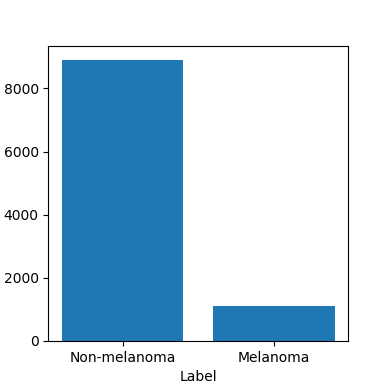
\includegraphics[width=0.5\textwidth]{figs/data_barplot.png}
    \caption{Bar plot of the distribution of the dataset's labels (melanoma or non-melanoma cases).}
    \label{fig:classimbalance}
\end{figure}

We correct this imbalance by oversampling the minority class, while also augmenting the total number of samples to $m' \approx 18000$ to increase the size of the dataset. That means we must augment the minority class by a factor of $\frac{\frac{m'}{2}}{|S_{min}|}$ and the majority class by a factor of $\frac{\frac{m'}{2}}{|S_{maj}|}$. For this augmentation we consider a set $T$ of possible transformations:

\begin{itemize}
    \item Horizontal flip
    \item Vertical flip
    \item 90º rotation
    \item 180º rotation
    \item 270º rotation
\end{itemize}

implemented by \verb|PIL.Image.transpose|\footnote{\url{https://pillow.readthedocs.io/en/stable/reference/Image.html\#PIL.Image.Image.transpose}} with the respective method:

\begin{itemize}
    \item \verb|PIL.Image.FLIP_LEFT_RIGHT|;
    \item \verb|PIL.Image.FLIP_TOP_BOTTOM|;
    \item \verb|PIL.Image.ROTATE_90|;
    \item \verb|PIL.Image.ROTATE_180|;
    \item \verb|PIL.Image.ROTATE_270|.
\end{itemize}

On principle, we did not consider transformations that change the color (e.g. contrast change, channel shift) or size (e.g. zoom) of features because it would unjustifiably allow the network to learn from these potentially misrepresenting features which even an expert human diagnosis would have trouble with.

The final available augmentations are all the $k$-combinations of the set $T$ for $k \in \{1, ..., |T|\}$, in other words all the possible ways in which you can combine the transformations from the set $T$.

\subsection{Split}

The number of variables in the future experiments would quickly lead to a combinatorial explosion of configurations, so to minimize the computational cost of the experiments a fixed validation scheme will be used rather than a cross validation scheme. To compensate for this lack of averaging over multiple folds of the data (which gives statistical confidence in the results), a fixed seed is set for every \ac{PRNG} as in code listing \ref{code:seed}, which in practice means parameters are initialized identically between experiments (providing some level of statistical confidence when making comparisons) and guarantees reproducibility.

\begin{listing}[ht]
\begin{minted}{python}
def seed():
    from random import seed
    seed(1)
    import numpy.random
    numpy.random.seed(2)
    from tensorflow import set_random_seed
    set_random_seed(3)
\end{minted}
\caption{Seed function that is called on every experiment to ensure reproducibility and similar conditions between experiments.}
\label{code:seed}
\end{listing}

The original training set from \ac{ISIC} 2018 is available for direct download, but the validation and test sets are kept private by the organization and are only used internally for reporting performance without actually releasing the data itself. As such, we will split the samples from the training set (which is available for download) into our own training, validation and test sets.

Augmentation, as described previously, results in 17810 samples which are split 85\%-15\% in a stratified fashion to maintain class balance within the splits into:

\begin{itemize}
    \item 15137 training samples, illustrated in figure \ref{fig:data_train};
    \item 2673 test samples, illustrated in figure \ref{fig:data_test}.
\end{itemize}

\begin{figure}[ht]
    \centering
    \includegraphics[width=0.6\textwidth]{../plots/data/train.png}
    \caption{Randomly-sampled images and respective labels of the train set.}
    \label{fig:data_train}
\end{figure}

\begin{figure}[ht]
    \centering
    \includegraphics[width=0.6\textwidth]{../plots/data/test.png}
    \caption{Randomly-sampled images and respective labels of the test set.}
    \label{fig:data_test}
\end{figure}

Since validation is intrinsically part of the training process itself, the validation set is a 15\% split from the training set obtained independently at the start of each training routine (also in a stratified fashion).

\section{Hardware}

Initially, computational resources from \ac{IEETA} were used in very early exploratory research:

\begin{itemize}
    \item Intel® Xeon® Processor E5-2640;
    \item NVIDIA Tesla K40c;
    \item NVIDIA Quadro K4000;
    \item 32GB DDR4 RAM.
\end{itemize}

However, given that it was shared between dozens of other researchers it was deemed not enough for a comfortable and flexible workflow because:

\begin{itemize}
    \item the little amount of memory almost wasn't enough to load the dataset into memory, especially during critically busy times;
    \item the NVIDIA Quadro K4000, with a compute capability of 3.0, was unsupported by the software stack which required a minimum compute capability of 3.7, leaving only a single NVIDIA Tesla K40c to work with.
\end{itemize}

More recently, \ac{LAR}, located in the Department of Mechanical Engineering at the University of Aveiro, has provided access to their deep learning research server codenamed Deeplar:

\begin{figure}[ht]
    \centering
    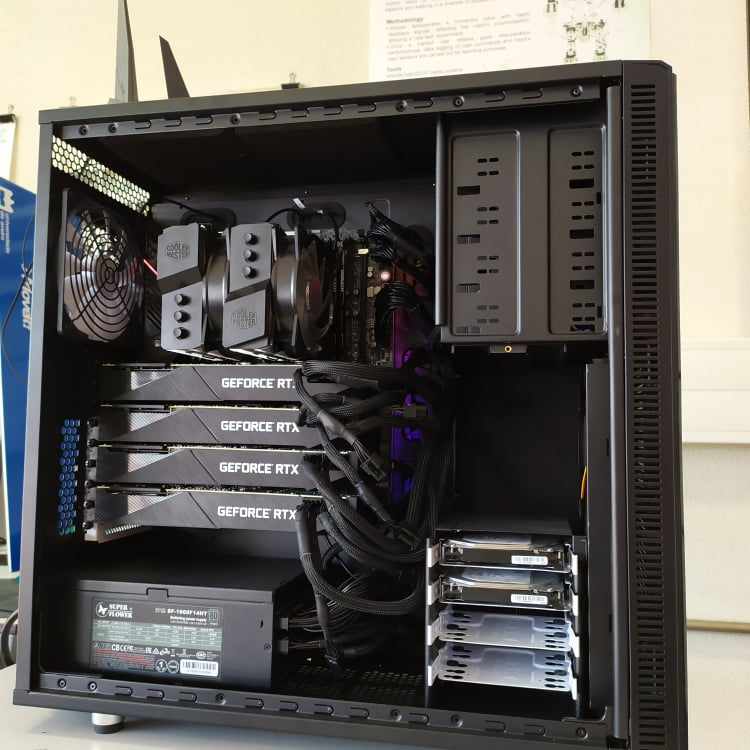
\includegraphics[width=0.4\textwidth]{figs/deeplar.jpg}
    \caption{Deeplar, the deep learning research server at \ac{LAR}}
    \label{fig:deeplar}
\end{figure}

\begin{itemize}
    \item AMD Ryzen™ Threadripper 2950X;
    \item Four NVIDIA GEFORCE® RTX 2080 Ti;
    \item 128GB DDR4 RAM.
\end{itemize}

The latter much more capable server (four state-of-the-art consumer \ac{GPU} and lots of \ac{RAM}) was effectively responsible for running this work's experiments.

\section{Software}

The deep learning research server Deeplar runs on openSUSE Tumbleweed 20191004\footnote{\url{https://software.opensuse.org/distributions/tumbleweed}}, a popular rolling-release GNU/Linux distribution. For interfacing with the \ac{GPU} it has installed CUDA 9.2 \footnote{\url{https://developer.nvidia.com/cuda-zone}} (NVIDIA GPU's proprietary language and API) and cuDNN 7.6.0 \footnote{\url{https://developer.nvidia.com/cudnn}} (a library for working with deep neural networks which most higher level frameworks rely on).

We used Miniconda\footnote{\url{https://docs.conda.io/en/latest/miniconda.html}} to install Conda\footnote{\url{https://conda.io/en/latest/}} which was used to manage a Python 3.6\footnote{\url{https://www.python.org/}} environment which was specifically required for compatibility with TensorFlow. Crucially, the following Python packages and specific versions were used for the development of most of the source code.

\begin{itemize}
    \item TensorFlow\footnote{\url{https://www.tensorflow.org/}} 1.12.0, of which we mostly use the \verb|tf.keras| API, for training and testing the various models;
    \item scikit-learn\footnote{\url{https://scikit-learn.org/}} 0.20.2 for some useful metrics and data splitting methods;
    \item NumPy\footnote{\url{https://numpy.org/}} 1.15.4 for various vector and matrix operations and Pillow\footnote{\url{https://pillow.readthedocs.io/en/stable/}} 5.4.1 for image handling and transformations because of this work's image preprocessing needs.
\end{itemize}
